\documentclass{article}
\usepackage{pdfpages}

\title{Team Liza \\ Milestone 5}
\author{Sam Kim \\ Kevin Geisler \\ Michael Williamson \\ Brian Collins}
\date{2-10-12}

\begin{document}

\maketitle
\newpage

\tableofcontents

\newpage

\section{Introduction}

\noindent   

Minecraft [1] is a sandbox computer game where players can create and remove blocks in a simulated world. 
These blocks can be arranged in a nearly unlimited number of ways and is only limited by the player's imagination.
 Despite being recently officially released, it has gained immense popularity with a user base exceeding 10 million people. \newline

\noindent Modifying Minecraft [1] has become increasingly popular, as a number of changes can be made to suit each user’s needs.
 There are currently two methods of modifying Minecraft [1]. Mods require a user to directly modify their game files in order to add 
or alter functionality in Minecraft [1]. For a server to effectively use a mod, the server requires each user to install that mod. On the 
other hand, plugins enable developers to make changes to Minecraft [1] without needing each user to directly modify the platform. 
Only the server needs to be modified. \newline 

\noindent A common way of introducing plugins to a Minecraft [1] server is to utilize a tool called Bukkit [2]. Bukkit wraps around the official
 server application and exposes an easy application programming interface (API) for developers to create plugins.  \newline

\noindent Bukkit [2] currently does not possess any means of testing, which makes debugging plugins a tedious process. Liza intends to 
provide a unit testing framework for plugin developers to programmatically test their code.  This document will briefly summarize the 
problem with the current system, and provide details on how Liza intends to solve them. This will be a compilation of all of the previous
 milestones, and include the need, features, requirements, and details about the development of the system.

\newpage

\section{Analysis Models}
\subsection{Domain Model}

This is the final design for the Liza Unit Testing Framework.  Our domain model shows the 
communication between the developers test code and Liza Classes which will interact
with Bukkit.  This shows the basic design of Liza without the complexity of the complete
Bukkit-Liza Class Diagram. \newline \newline

\noindent The diagram is depicted below:

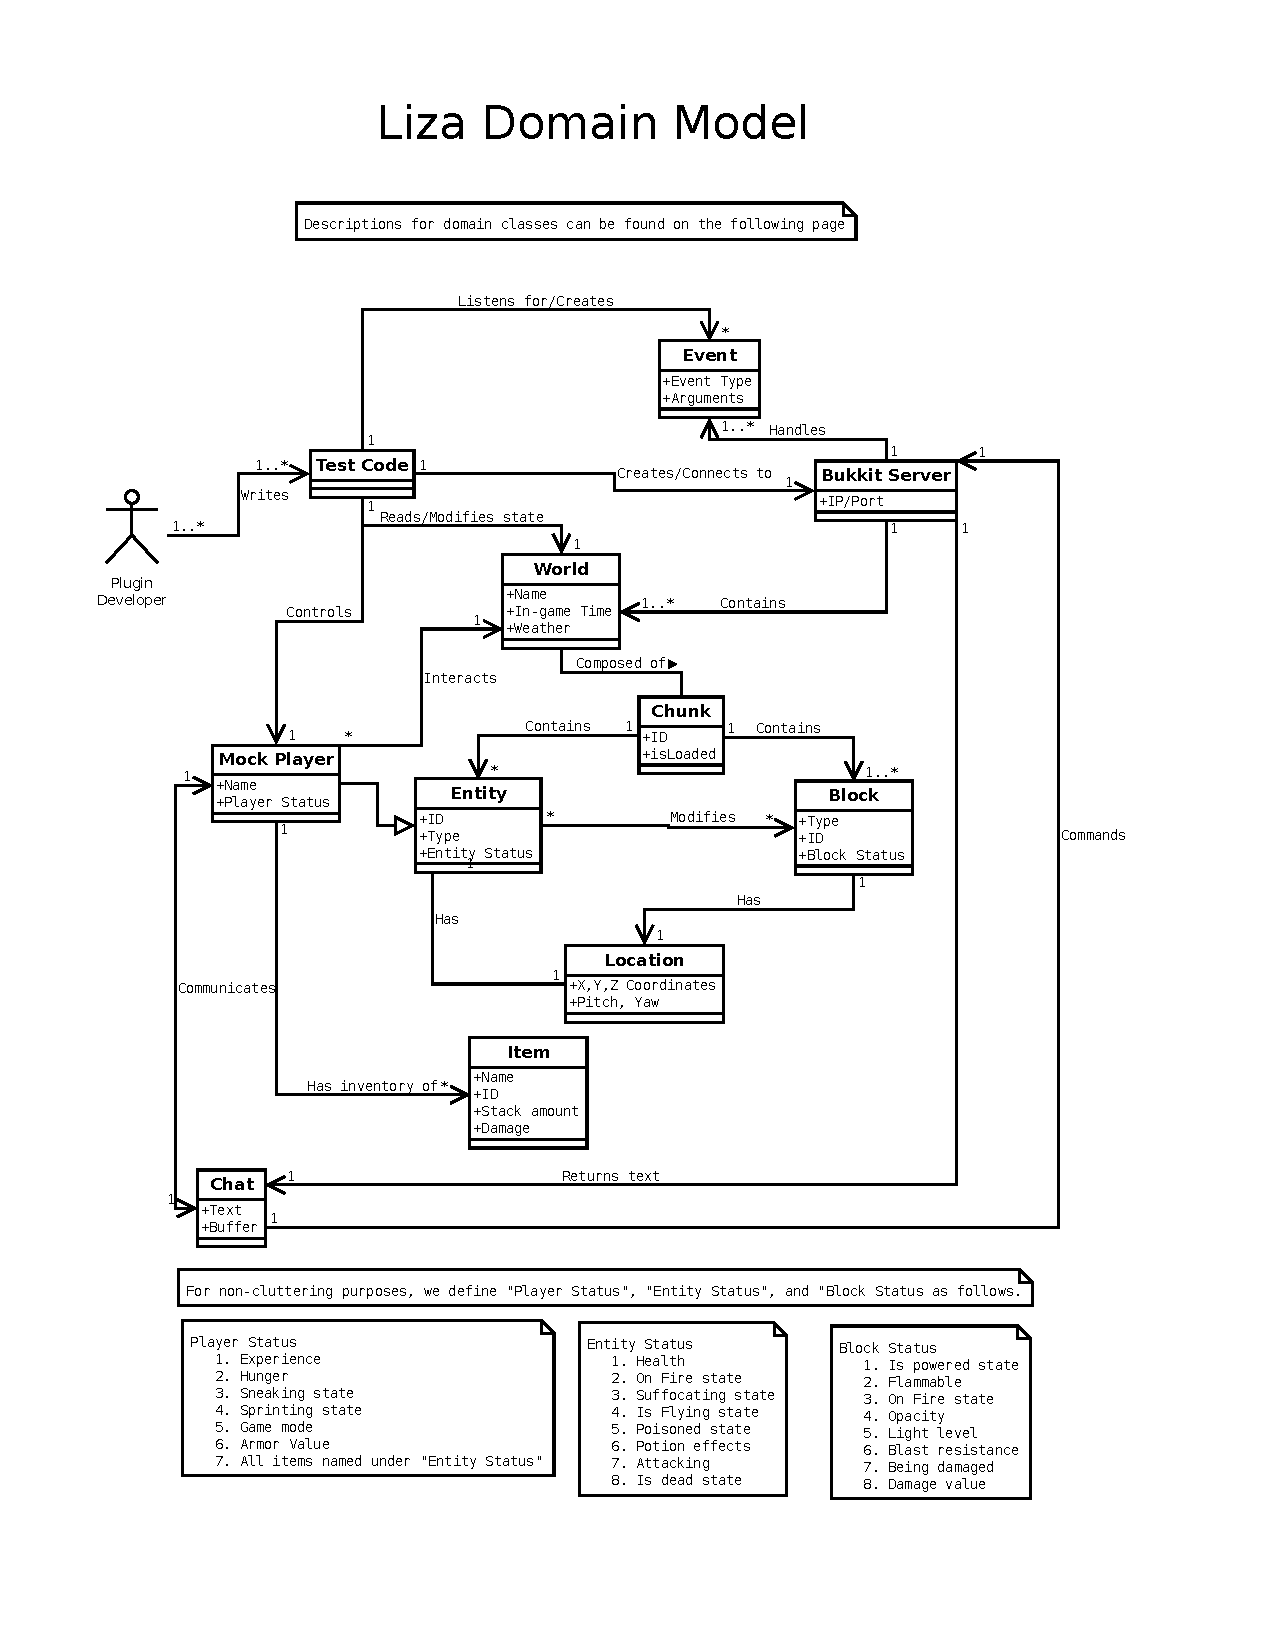
\includepdf[pages={-}]{DomainModel.pdf}

\newpage

\subsection{Activity Diagram}

\noindent   This diagram shows how the Developer's test code, the Liza interface, and Bukkit interactall together.
There is a large amount of activity that goes through a massive loop, shown in the rectangular box.  This loop
is the main guts of what Liza does when running.

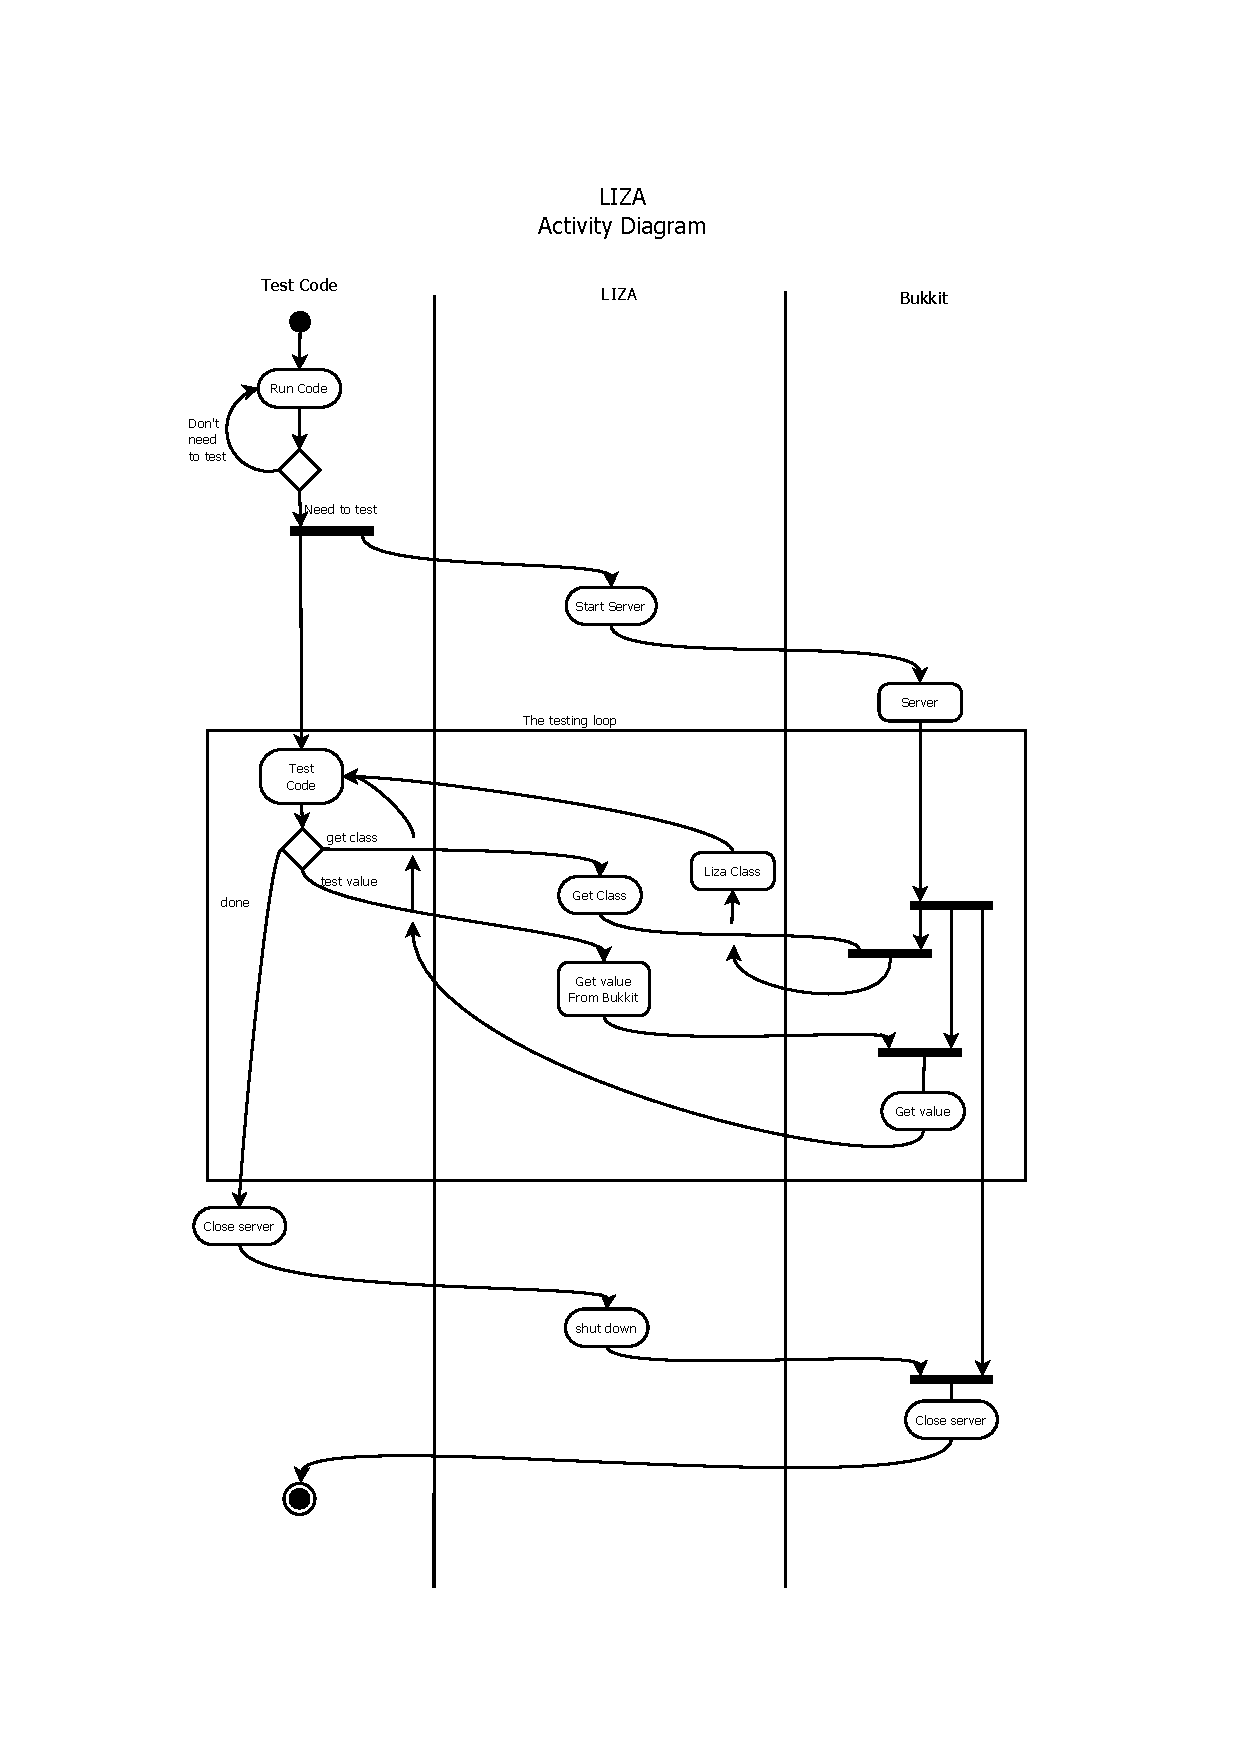
\includepdf[pages={1-1}]{LizaActivity.pdf}

\newpage

\section{Logical Architecture}
\subsection{System Sequence Diagrams (SSD)}

Description:  \newline

There are many SSDs that will apply to this project -- one for each assertion. 
However, each of these will follow the exact same format. Instead, we
produced a single SSD that details the flow of a test case that a developer may
write.  This includes general exception cases and alternate paths which could be
produced.  \newline \newline

\noindent  The SSD is shown below:

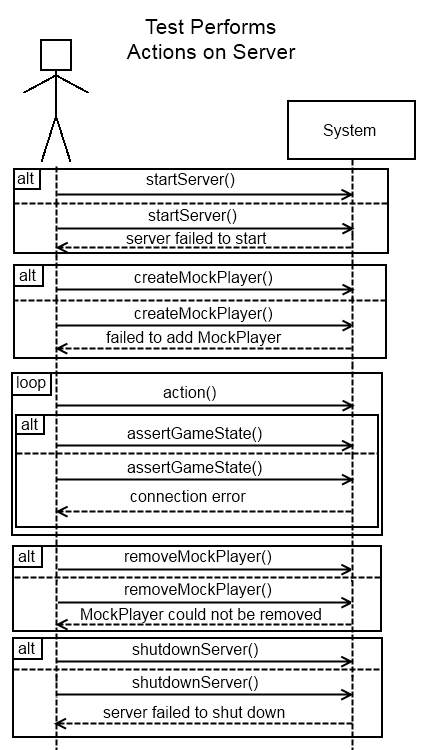
\includegraphics{ssd}


\subsection{Operational Contracts (OC)}

There will be a controller in Liza to start the server that it will control.
 Here is an operational contract which describes the startup process.:  \newline

\textbf{Operation name:} startServer() 
\newline \indent
\textbf{Cross-References:} SSD1 
\newline  \indent
\textbf{Preconditions:} LizaCraftController has been created.
\newline  \indent
\textbf{Postconditions: }
	\begin{enumerate}
		\item CraftBukkitThread was created.
		\item CraftBukkitThread was run
		\item CraftServer object was retrieved from CraftBukkitThread
		\item EventListener was created
		\item Association between EventListener and CraftServer established
	\end{enumerate}•

\subsection{Package Diagram}

There exists a degree of separation between our system and Bukkit, in the
sense that our system interacts with Bukkit, yet Bukkit is not aware of our
system. However, all of the classes in our system will all belong to the same
package, due to the high amount of interaction between classes. Because
of this, a package diagram is not applicable.  However, we have included a 
diagram which depicts the relationship between Liza and Bukkit in general.
For each Bukkit class that is relavent, Liza will extend a new interface and 
create a new LizaCraft class that will implement it. \newline 

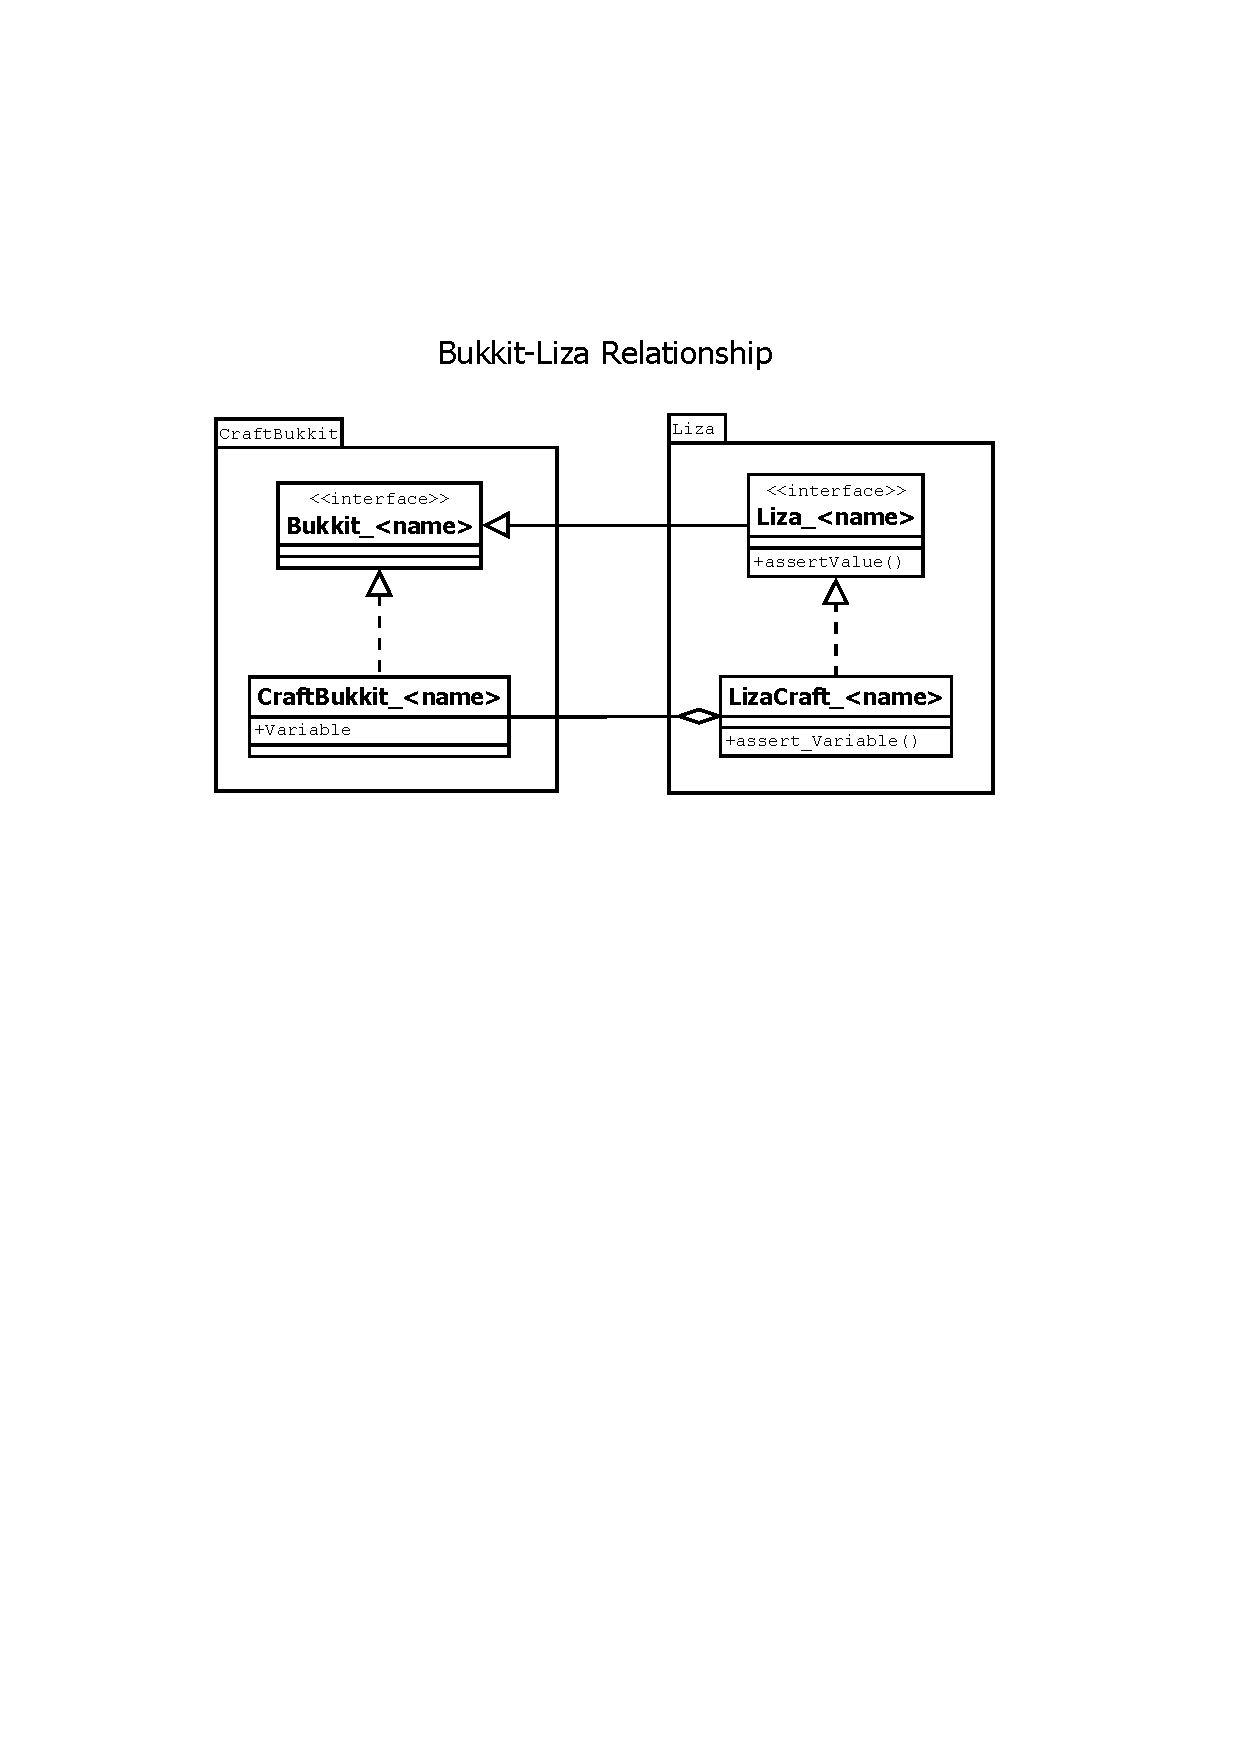
\includepdf[pages={-}]{Bukkit-Liza-Relationship.pdf}

\subsection{Class Diagram}

Description:
\newline

\noindent
Bukkit has two main layers: Bukkit, which is a collection of interfaces that
a plugin developer utilizes, and CraftBukkit, which is the implementation
of those interfaces. Our system will mirror this design. There is Liza, which
is a set of interfaces that inherit the Bukkit interfaces, and LizaCraft, which
is the implementation of the Liza interfaces and extends the CraftBukkit classes.
By extending the existing Bukkit and CraftBukkit, we present the API that
the developers are accustomed to, along with any new methods that may
be of use for testing, such as asserting properties. 
\newline

\noindent
There are a few new classes, however. LizaMockPlayer and its associated
implementation represent the automated player that the developer
commands. LizaMockPlayer and LizaPlayer are separated because the
latter asserts properties of any player, while the former controls only
the automated player.
\newline

\noindent
LizaListener and LizaEventExecutor handle the listening and spoofing of
events, respectively. 
\newline

The diagram is found on the following pages.
\newline

\newpage
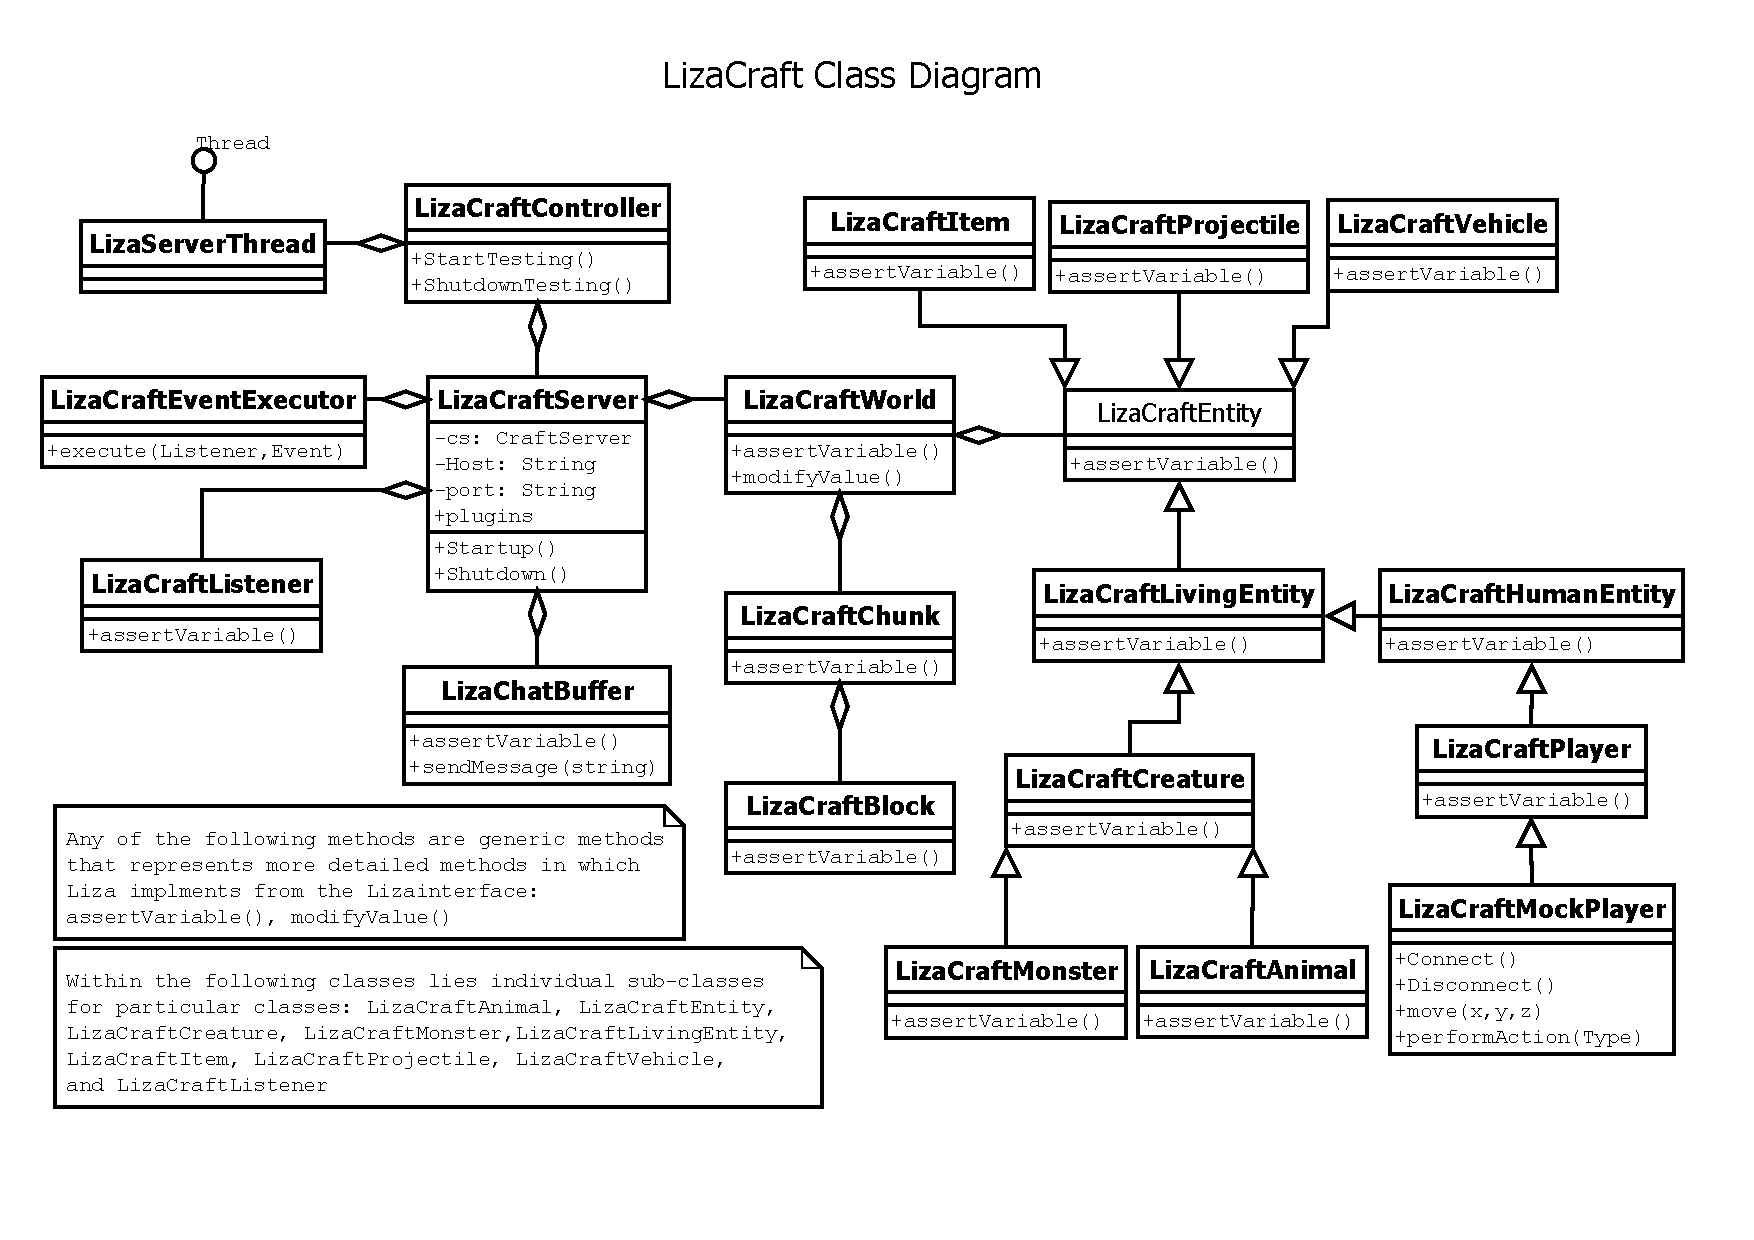
\includepdf[pages={-}]{LizaClassDiagram.pdf}

\newpage

\section{Gang of Four Patterns}

In this section, we will discuss which of the Gang of Four patterns
apply to our design.

	\subsection{Adapter}

	As Liza is an extension of Bukkit, we felt it necessary to mirror 
	Bukkit's design to our own. This involved making Liza versions of many
	classes, as noted in the package overview diagram. To reduce coupling
	with Bukkit, we instead chose to make each of our classes an adapter
	to the appropriate Bukkit class. 

	\subsection{Fa\c{c}ade}

	Liza is responsible for starting up the server, retrieving the server object and
	enabling event listening, among other tasks. These are rather complex
	control sequences. Therefore, to hide this away, we've created a $LizaTestModule$
	class, an application of the Fa\c{c}ade pattern. The code to the developer simply
	becomes

	\begin{verbatim}
	LizaTestModule test = new LizaTestModule();
	test.start();
	test.enableEvents();
	// code work here
	test.disableEvents();
	test.end();
	\end{verbatim}•

	\subsection{Observer}

	Minecraft, and by association Bukkit, has nearly every action driven
	by player input. The game handles these actions by using event handlers.
	
	We feel that a test developer will also be interested in these events.
	Therefore, we have added the $LizaPlugin$ class. It itself is an observer --
	it is able to register events with Bukkit's event dispatcher, and gets notified 
	when such events occur. 

	However, we also open up the test developer to observe
	the $LizaPlugin$. A developer will register an event to listen for through
	the class. Then the $LizaPlugin$ will register that event to Bukkit. When
	the event occurs, we relay that event to the developer.

\newpage
\section{Acceptance Test Plan}

\noindent It is vital for any testing framework to work reliably. Because of this, we will be using Bukkit's  
API to assert that the mock player's states are correct through a testing plugin. In general, we will be using
Bukkit's API (which is assumed to be correct) to check against Liza's values. For control’s sake, the test plugin
will be run on a world that is generated to be completely flat, with no obstacles or pitfalls, and natural entity 
spawning disabled. If a test case would require such things, the testing plugin will be able to spawn them in manually.
\newline \newline \noindent
In the descriptions, the terms “testing plugin” (that will be used to test Liza) and “Bukkit” will be used interchangeably.
\newline \newline \noindent
The Acceptance Test Plan is as shown below:


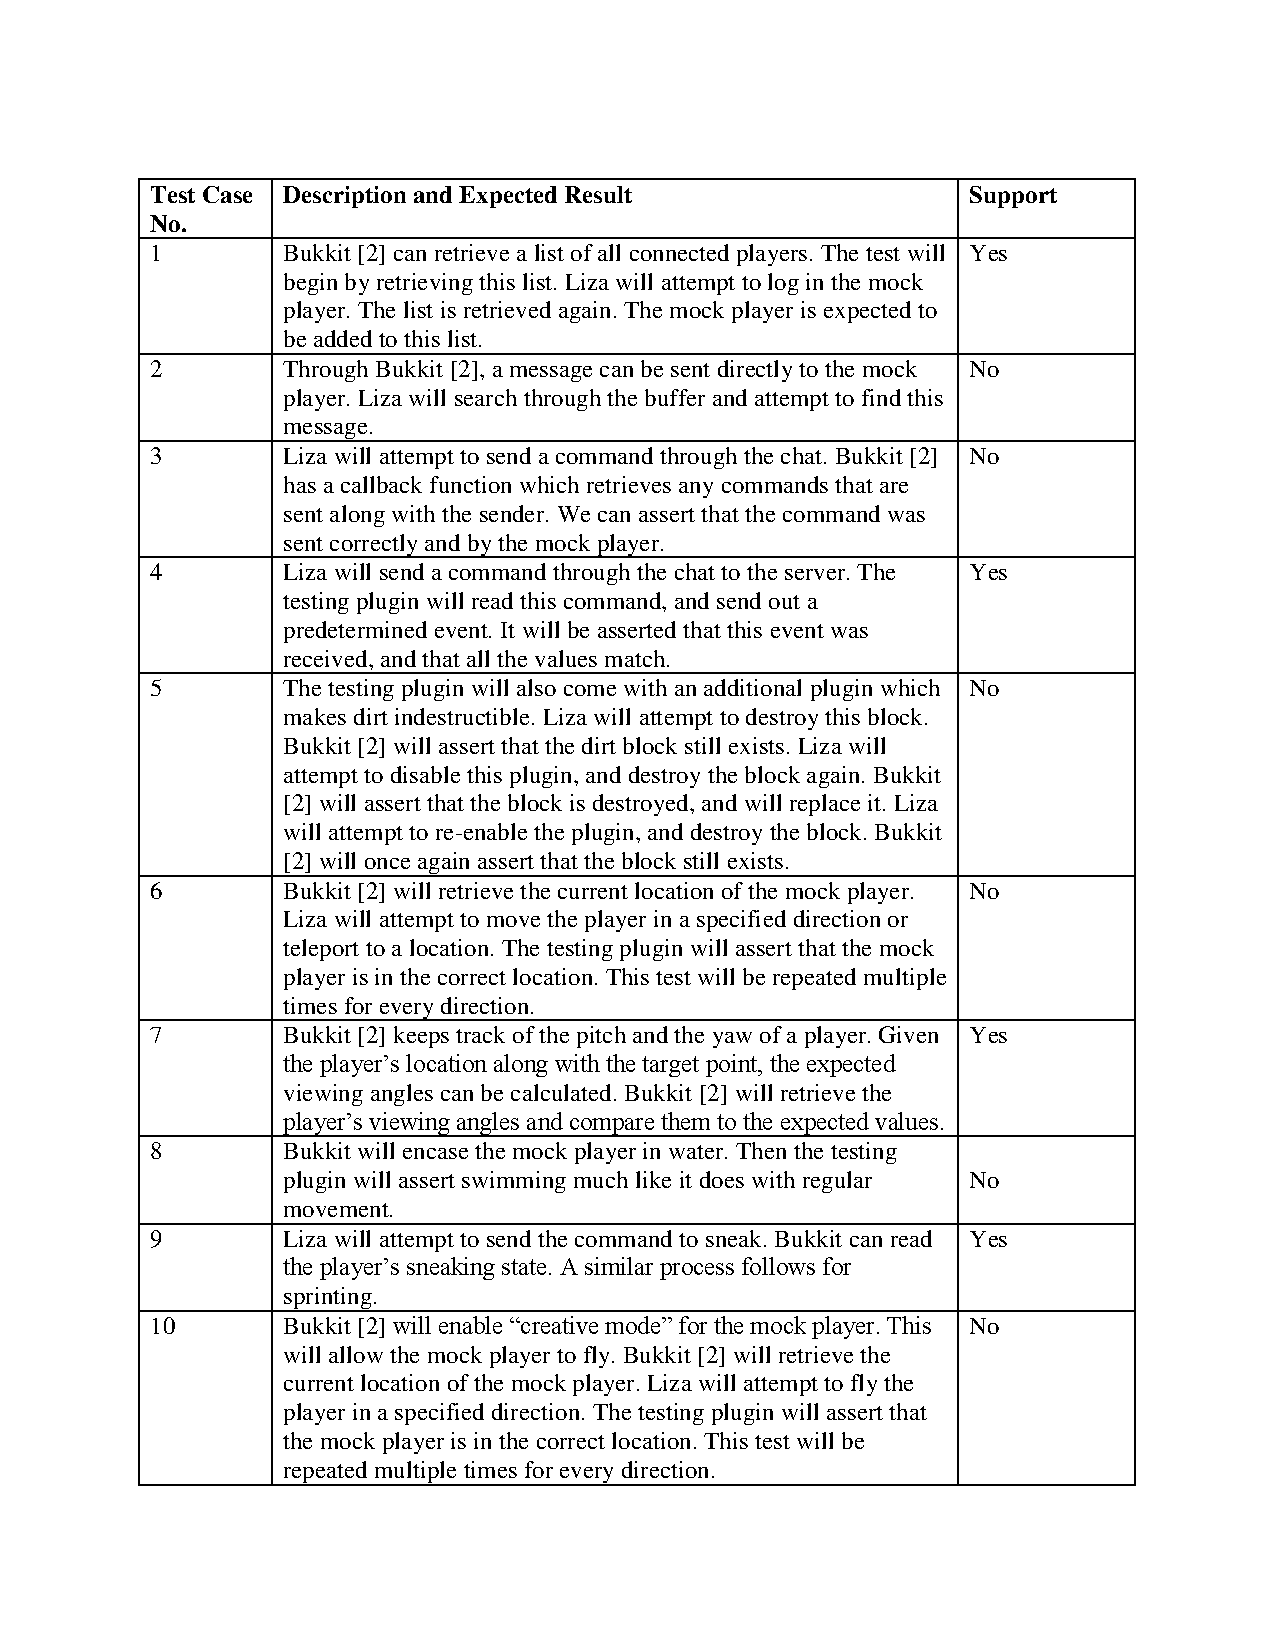
\includepdf[pages={-}]{TestCases.pdf}


\end{document}